\documentclass{article}
\usepackage{tikz}
\usepackage{amsmath}
\usepackage{geometry}
\geometry{a4paper,layout=a4paper,left=2cm,right=2cm,top=2cm,bottom=2cm}

\usepackage{pgfplots}

\begin{document}
	\begin{tikzpicture}
		\draw (0,0) -- (1,2);
	\end{tikzpicture}
	\begin{tikzpicture}
		\draw[scale=2] (0,0)--(1,2) ;
		\draw [->](0,0)--(2,0);
		\draw[<-> ] (3,0)--(4,0)--(5,2);
	\end{tikzpicture}

	\begin{tikzpicture}
		\draw[<-,thick,blue,dashed] (0,4)--(0,0);
		\draw[->,thin,green,double] (0,0)--(4,0);
	\end{tikzpicture}

	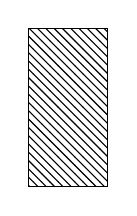
\begin{tikzpicture}
		\usetikzlibrary{patterns}
		\draw[pattern=north west lines] (0,0) rectangle (1,2);
	\end{tikzpicture}

	\begin{tikzpicture}
		\draw[ thin,gray,->] (-0.2,0)--(4,0) node[below]{$x$};
		\draw[thin,gray,->] (0,-0.2)--(0,4)node[left]{$y$};
		\draw[thin,gray,->] (0,0,-0.2)--(0,0,4)node[left]{$z$};
		\draw[very thin,gray] (-0.1,-0.1) grid (3.9,3.9);
	\end{tikzpicture}
	\tikz{\fill[red] (0,0) rectangle (2,1);
		\fill[ nearly transparent,green] (0,0) rectangle (1,2);}
\end{document}